\section{Theorie}

\subsection{organische Szintillatoren}

Szintillatoren sind  Materialien die bei bestrahlung mit energiereichen Photonen oder geladenen Teilchen angeregt werden und die Anregungsenergie in Form von Licht wieder abgeben. Organische Szintillatoren bestehen wie der Name schon vermuten lässt vorwiegend aus Kohlenstoff, Wasserstoff, Sauerstoff und Stickstoff wie es auch in z.B. menschlichem Gewebe der Fall ist. Es liegt daher nahe Detektoren auf Basis organischer Szintillatoren für die Dosismessung im Strahlenschutz zu verwenden. Organische Szintillatoren bestehen typischerweise aus zwei Komponenten: Einem primären Fluoreszenzstoff (z.B. auf Basis von Polyvinyltoluol) und einem \glqq Wellenlängenschieber \grqq{} (z.B. POPOP) da die vom primären Fluoreszenzstoff abgegebenen UV-Strahlen in den meisten durchsichtigen Materialien eine nur sehr geringe Reichweite besitzen.

\subsection{Wechselwirkung von Photonen mit Materie}

Obwohl Photonen in vieler Weise mit Materie wechselwirken können sind für diesen Versuch nur zwei Prozesse von wesentlicher Bedeutung: Die Compton-Streuung und der Photoeffekt. In den folgenden Abschnitten werden beide näher erläutert.

\subsubsection{Photoeffekt}

Der Photoeffekt beschreibt die Anregung von Elektronen durch Absorption eines Photons.
Für den HPGe-Detektor ist vor allem der innere photoelektrische Effekt von Bedeutung. Er beschreibt die Zunahme der Leitfähigkeit eines Halbleiters durch Bildung von nicht aneinander gebundenen Elektron-Loch-Paaren. Der HPGe-Detektor besteht aus einem hochreinen Germanium-Kristall der zwischen einem $n^{+}$ Kontakt (typ. durch Lithium-eindiffusion) am positiven Spannungspol und einem $p^{+}$ Kontakt (typ. durch Bor-implantation) am negativen Spannungspol sitzt; Der Detektor insgesamt entspricht einer Halbleiterdiode in Sperrichtung. Trifft ein Photon auf den Detektor und erzeugt ein Elektron-Loch-Paar werden durch die anliegende Spannung Elektron und Loch abgesaugt und bilden so einen detektierbaren Verschiebungsstrom. Dafür muss das einfallende Photon natürlich genügend Energie besitzen um die Bandlücke zu überwinden (Für Germanium \SI{0.67}{\electronvolt}), praktisch jedoch deutlich mehr um das Siganl-Rausch-Verhältnis groß genug zu bekommen. So werden bei einfallenden Photonen von \SI{1}{\mega\electronvolt} etwa \num{3e5} Elektron-Loch-Paare erzeugt \cite{HPGe-Detektor}. Da bei Raumtemperatur eine ständige thermische Anregung der Elektronen enormes Signalrauschen verursachen würde ist eine Abkühlung mit flüssigem Stickstoff notwendig.
Für den zu kalibrierenden Detektor ist vor allem der äußere photoelektrische Effekt von Bedeutung, genauer für den Photoelektronenvervielfacher (Abb. \ref{theorie_PEV}).

\begin{figure}[ht]
	\centering
  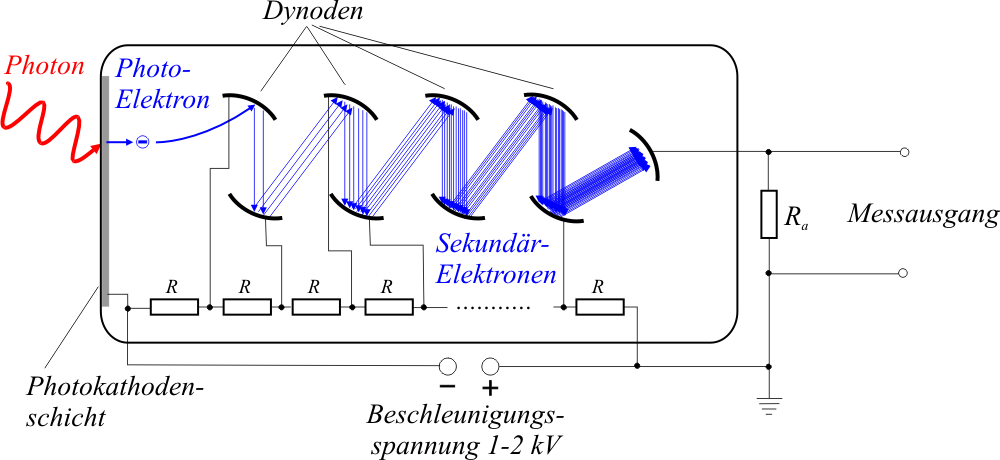
\includegraphics[width=0.85\textwidth]{images/Photomultiplier_schema_de.png}
	\caption{Schematik Photoelektronenvervielfacher}
	\label{theorie_PEV}
\end{figure}

Dort werden durch das Szintillationsphoton Elektronen aus einer Photokathode ausgeschlagen, durch angelegte Spannung zur ersten Dynode beschleunigt wo sie mit der gewonnenen kinetischen Energie weitere Elektronen auschlagen. Dieser Prozess wird einige male wiederholt bis ein messbarer elektrischer Impuls an der Anode entstehen kann.

\subsubsection{Compton-Streuung}

\subsection{Weitwinkel-Compton-Koinzidenz-Methode}
